\documentclass[11pt,a4paper]{article}

\usepackage[a4paper,margin=2.5cm]{geometry}
\usepackage[T1]{fontenc}
\usepackage[utf8]{inputenc}
\usepackage{lmodern}
\usepackage{amsmath}
\usepackage{amssymb}
\usepackage{graphicx}
\usepackage{booktabs}
\usepackage{siunitx}
\usepackage{float}
\usepackage{subcaption}
\usepackage{natbib}
\usepackage{hyperref}
\usepackage{enumitem}
\usepackage{setspace}

\hypersetup{
  colorlinks=true,
  linkcolor=blue,
  citecolor=blue,
  urlcolor=blue
}

\sisetup{
  detect-all,
  separate-uncertainty=true,
  table-number-alignment=center,
  group-digits=false
}
\DeclareSIUnit\angstrom{\text{\AA}}

\title{Finding the Unit-Cell Parameter of an Unknown Powder\\[0.4em]\large Technical XRD Report}
\author{[Name]\\Lab partners: [Names]}
\date{[Date]}

\begin{document}

\maketitle
\begin{abstract}
This report analyzes an unknown powder sample using X-ray diffraction under the assumption that the dominant phase has a cubic unit cell. The experimental diffractogram was indexed by comparing measured $\sin^2(\theta)$ ratios with allowed cubic reflection sequences, and candidate crystal structures were checked against simulated powder diffractograms from the American Mineralogist Crystal Structure Database (AMCSD). The strongest reflections were observed near \SI{28.48}{\degree}, \SI{47.31}{\degree}, \SI{56.16}{\degree}, and \SI{69.17}{\degree}. From these strong reflections, the best-fit lattice parameter was found to be $a = \SI{5.4276}{\angstrom} = \SI{0.54276}{\nano\meter}$. The dominant pattern is most consistent with a cubic diamond-type diffraction pattern, and comparison with simulated candidates suggests that silicon is the most plausible identification, while ZnS remains a useful structural comparison.
\end{abstract}

\section{Introduction}
X-ray diffraction (XRD) is a non-destructive method for probing crystal structure by measuring the angles at which X-rays are diffracted by a periodic atomic arrangement. In this experiment, the sample was presented as an unknown powder with a cubic unit cell, which reduces the indexing problem to determining the allowed cubic reflection sequence and the corresponding lattice parameter $a$ \citep{onnink2026}.

The aim of this report is to determine the cubic unit-cell parameter of the unknown powder from its diffractogram and use that result, together with peak indexing and simulated reference patterns, to identify the most likely crystal structure and material.

\subsection{Theory}
When X-rays are scattered by parallel crystal planes separated by a distance $d$, constructive interference occurs when Bragg's law is satisfied:
\begin{equation}
  n \lambda = 2 d \sin\theta
\end{equation}
where $\lambda$ is the X-ray wavelength, $\theta$ is the diffraction angle, and $n$ is the diffraction order \citep{bragg1913}.

For a cubic crystal,
\begin{equation}
  \frac{1}{d_{hkl}^2} = \frac{h^2+k^2+l^2}{a^2}
\end{equation}
so the unit-cell parameter can be calculated from
\begin{equation}
  a = d_{hkl}\sqrt{h^2+k^2+l^2}.
\end{equation}
This means that once a reflection is assigned a value of $N = h^2 + k^2 + l^2$, the corresponding $a$ value can be calculated directly. In practice, the measured ratios of $\sin^2(\theta)$ are compared with the allowed integer sequences for cubic lattices to test candidate indexing schemes.

\begin{figure}[H]
  \centering
  \fbox{\parbox[c][0.18\textheight][c]{0.82\textwidth}{\centering
  Replace with your own hand-drawn Bragg's law schematic showing constructive and destructive interference, the spacing $d$, the angle $\theta$, the wavelength $\lambda$, and the factors affecting peak intensity.}}
  \caption{Placeholder for the Bragg's law schematic required by the lab assignment.}
  \label{fig:bragg-placeholder}
\end{figure}

\section{Experimental Method}
\subsection{Diffractometer Set-up}
The measurement was a powder XRD scan in reflection geometry using Cu $K\alpha$ radiation with $\lambda = \SI{1.5406}{\angstrom}$. The raw dataset was provided as an exported XY file and contains \num{3805} points from \SI{25.026}{\degree} to \SI{74.974}{\degree} in $2\theta$, with a constant step size of approximately \SI{0.01313}{\degree}. The report structure here follows the style of the provided technical report reference, but the analysis and wording are based on our own dataset and calculations.

The original diffractometer settings were not embedded in the exported XY file, so tube current, generator voltage, slit settings, and detector model should be added from the lab notes if they are available. What is certain from the analysis is that the scan was carried out with Cu $K\alpha$ radiation and covered the angular range needed to capture the dominant cubic reflections.

\begin{figure}[H]
  \centering
  \fbox{\parbox[c][0.18\textheight][c]{0.82\textwidth}{\centering
  Replace with your own hand-drawn or redrawn schematic of the powder diffractometer, including source, incident optics, sample, goniometer, receiving optics, and detector.}}
  \caption{Placeholder for the experimental setup schematic required by the lab assignment.}
  \label{fig:setup-placeholder}
\end{figure}

\subsection{Measurement Procedure}
The unknown powder was measured as intensity versus $2\theta$ and exported as a two-column XY dataset. The usable scan range extended from \SI{25.026}{\degree} to \SI{74.974}{\degree}. Because only the processed XY file was available during the present write-up stage, the description here focuses on the analysis that can be reproduced directly from the exported data.

\subsection{Processing}
The raw diffraction data were analyzed with a custom Python workflow. Peak positions were extracted from the diffractogram, converted to $d$ spacings using Bragg's law, and compared through $\sin^2(\theta)$ ratios and $1/d^2$ ratios to allowed cubic reflection sequences. Both FCC- and BCC-type indexing were considered. We then simulated candidate powder patterns from AMCSD CIF files and compared those to the experimental peak positions and relative intensities using a custom Python script with Matplotlib for plotting \citep{downs2003,amcsd,python,hunter2007}.

\section{Results}
\subsection{Experimental Diffractogram}
Figure~\ref{fig:full-pattern} shows the experimental XRD pattern over the measured angular range. The four dominant reflections occur near \SI{28.47}{\degree}, \SI{47.31}{\degree}, \SI{56.16}{\degree}, and \SI{69.17}{\degree}. Small local maxima are visible near \SI{33.32}{\degree} and \SI{59.16}{\degree} in the zoomed views of Figure~\ref{fig:weak-peaks}, but these features are close to the noise level and were not treated as reliable peaks in the final indexing.

\begin{figure}[H]
  \centering
  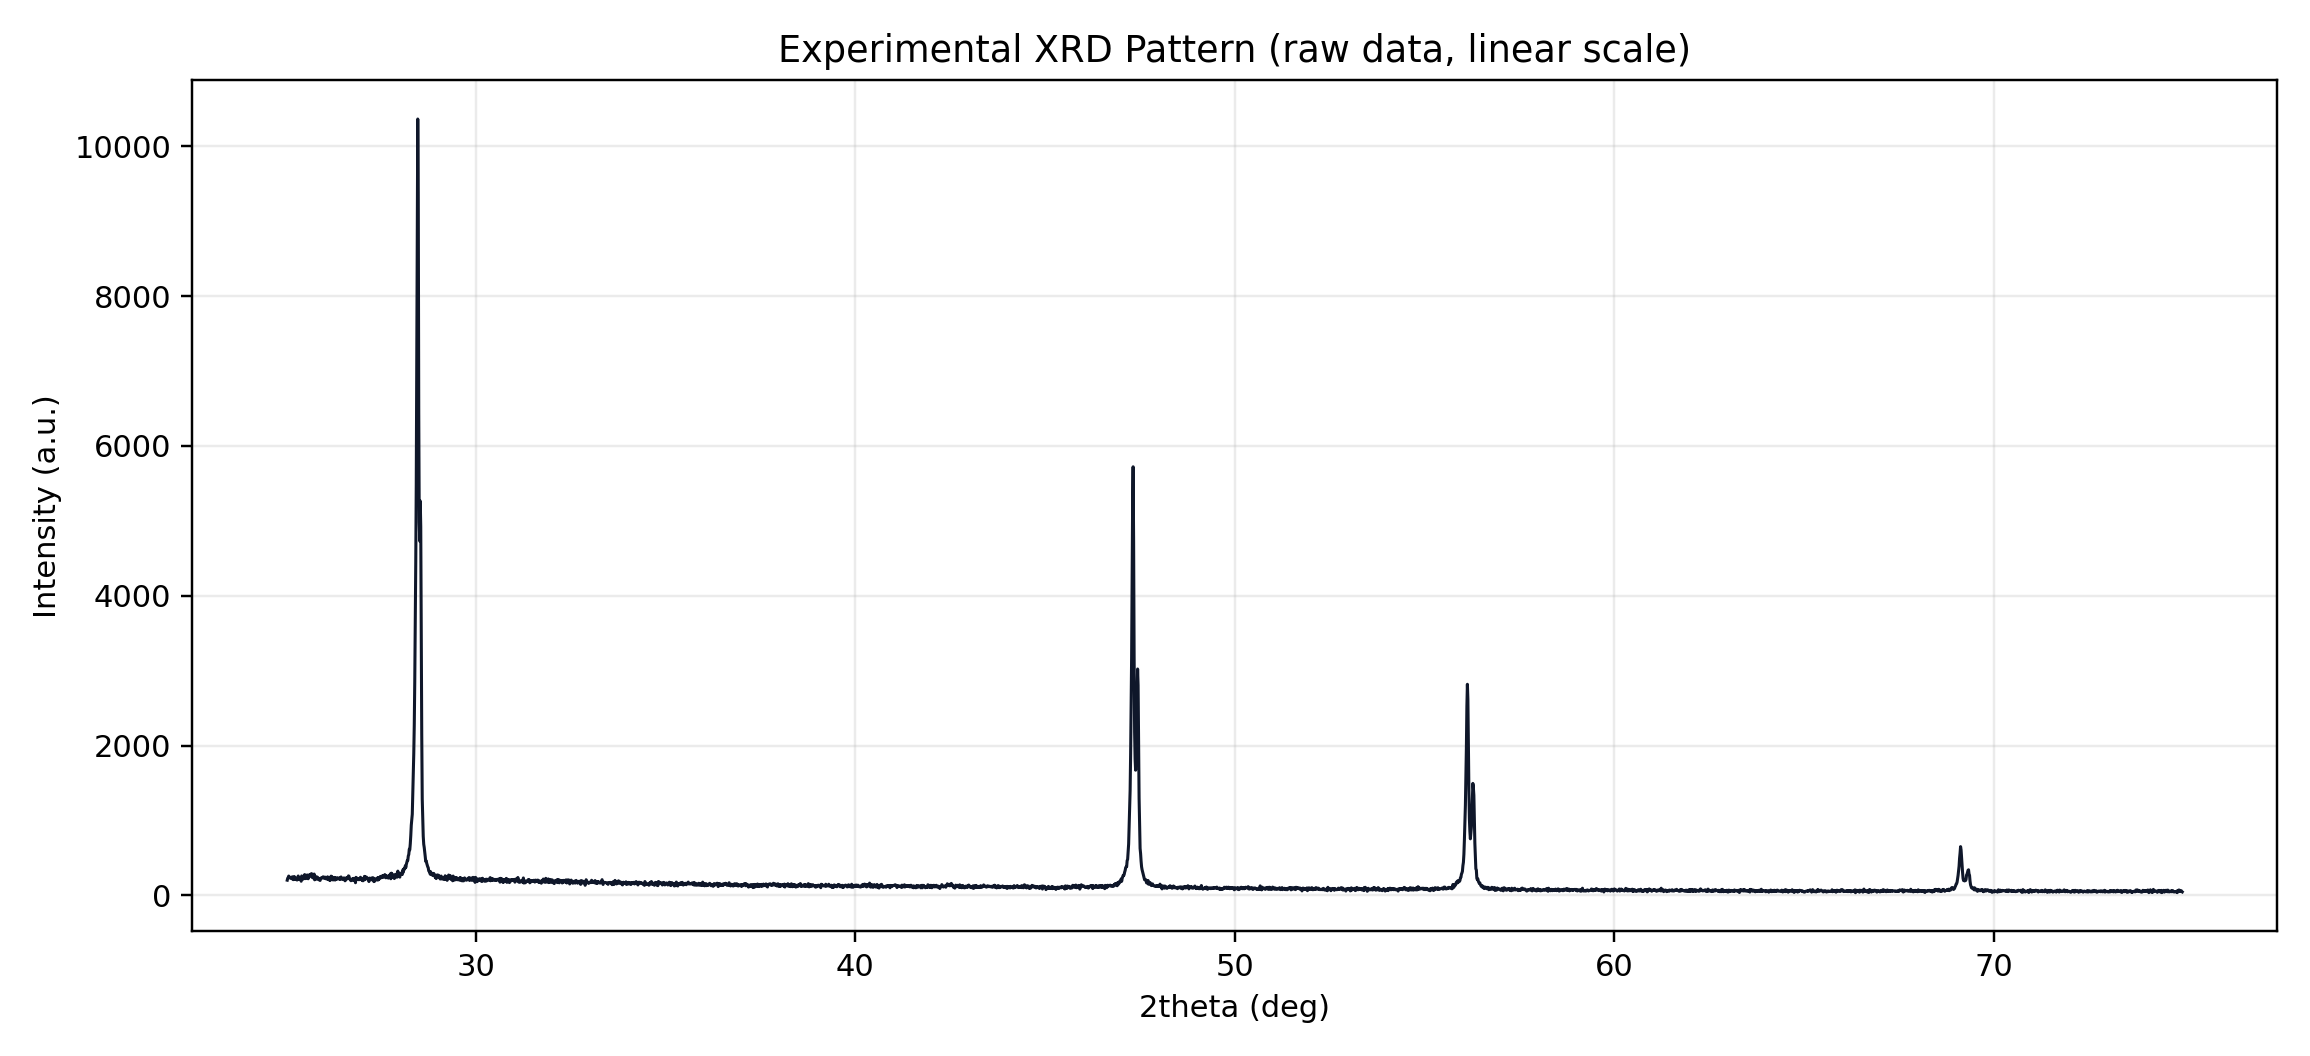
\includegraphics[width=0.86\textwidth]{figures/gr3_raw_full_linear.png}
  \caption{Experimental powder XRD pattern of the Group 3 sample.}
  \label{fig:full-pattern}
\end{figure}

\begin{figure}[H]
  \centering
  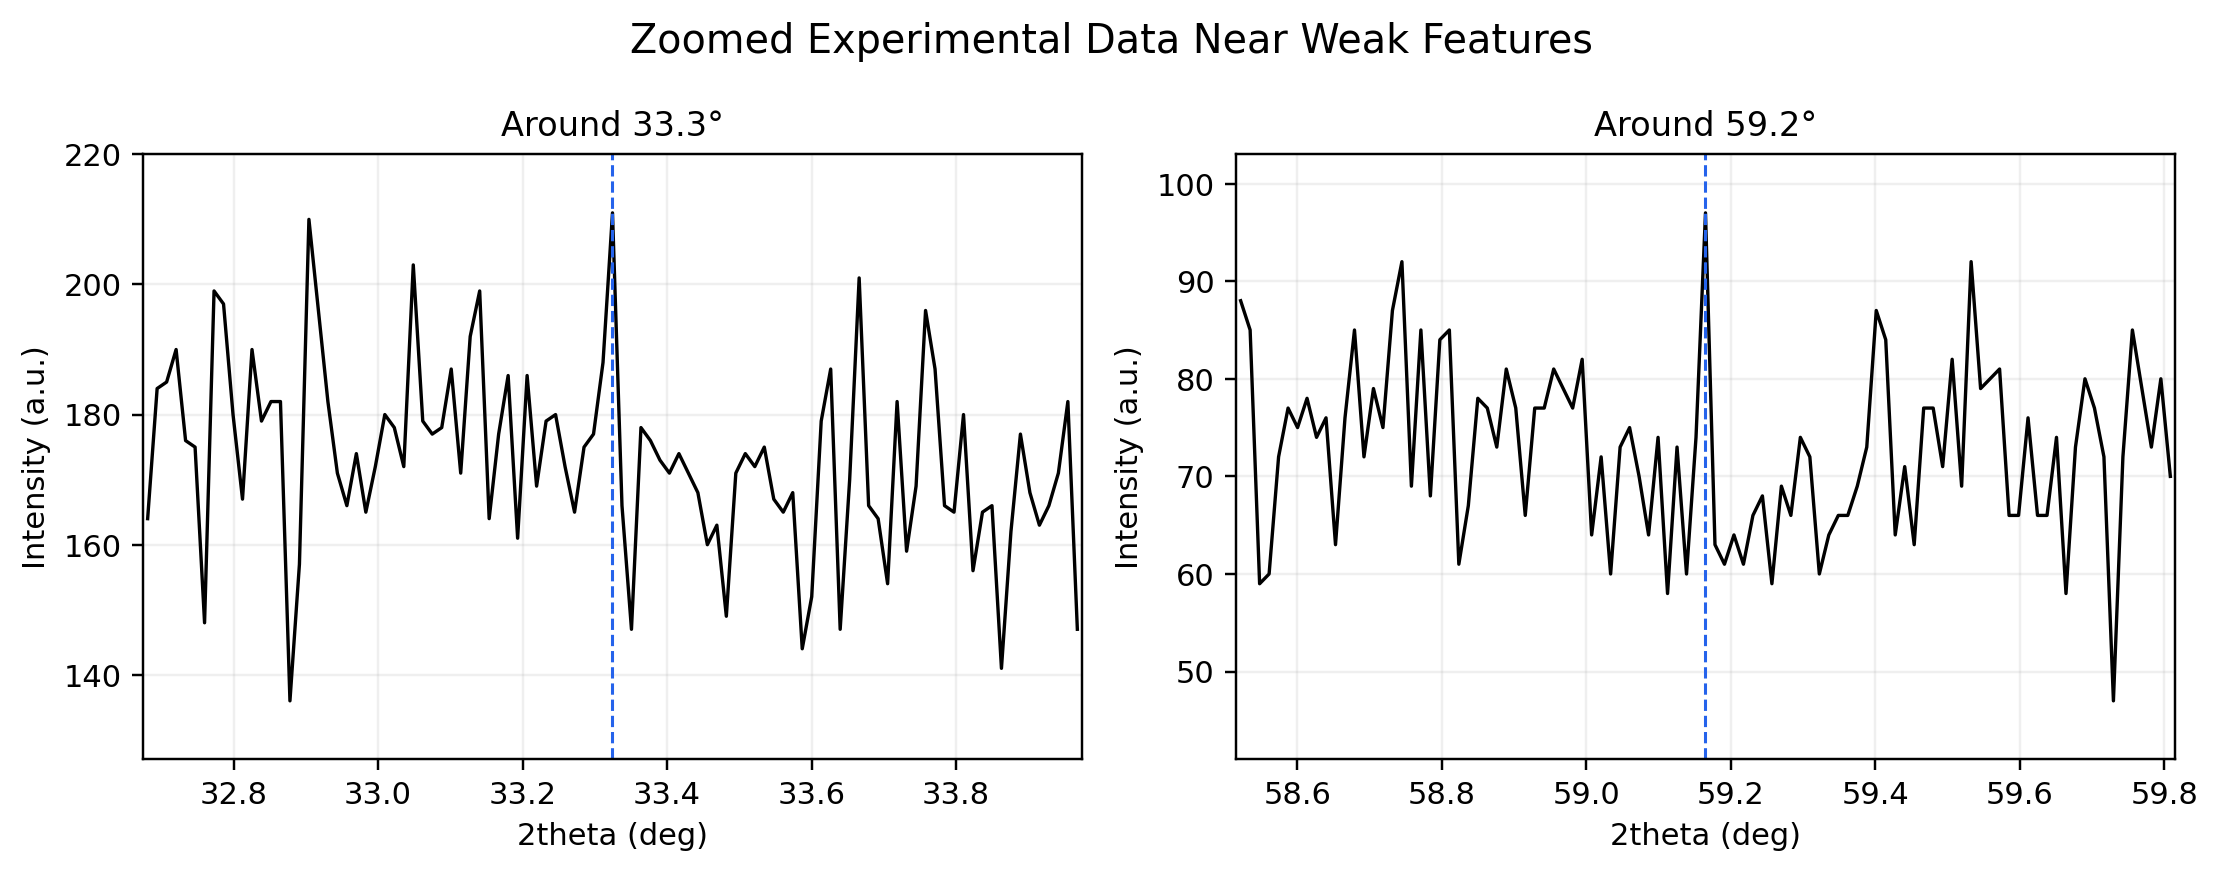
\includegraphics[width=0.94\textwidth]{figures/gr3_weak_peaks_simple.png}
  \caption{Zoomed raw-data views around the weak features near \SI{33.32}{\degree} and \SI{59.16}{\degree}.}
  \label{fig:weak-peaks}
\end{figure}

\subsection{Calculation of the Unit-Cell Parameter}
We started by assuming that the first strong peak at \SI{28.4794}{\degree} corresponds to the $(111)$ reflection, so $N = h^2+k^2+l^2 = 3$. This assumption was then tested against the measured $\sin^2(\theta)$ ratios of the remaining strong peaks.

For the first peak,
\begin{align}
  2\theta &= \SI{28.4794}{\degree}, \\
  \theta &= \SI{14.2397}{\degree}, \\
  d &= \frac{\lambda}{2\sin\theta} = \frac{\SI{1.5406}{\angstrom}}{2\sin(\SI{14.2397}{\degree})} = \SI{3.1316}{\angstrom}, \\
  a &= d\sqrt{3} = \SI{5.4240}{\angstrom}.
\end{align}

The full indexing table is shown in Table~\ref{tab:indexing}. The strong-peak ratios are close to the sequence $3,8,11,16$, which is consistent with a diamond-type cubic structure and incompatible with BCC indexing. If the first peak were BCC $(110)$, the later peak ratios should follow approximately $2.000$, $3.000$, and $4.000$, which does not match our measured ratios of $2.6605$, $3.6617$, and $5.3248$.

\begin{table}[H]
  \centering
  \caption{Peak indexing and unit-cell calculations for the Group 3 sample.}
  \label{tab:indexing}
  \begin{tabular}{cccccccc}
    \toprule
    Peak & $2\theta$ (\si{\degree}) & $d$ (\si{\angstrom}) & $1/d^2$ (\si{\per\angstrom\squared}) & Ratio & $N$ & $hkl$ & $a$ (\si{\angstrom}) \\
    \midrule
    1 & 28.4794 & 3.1316 & 0.1020 & 1.0000 & 3  & (111) & 5.4240 \\
    2 & 47.3083 & 1.9199 & 0.2713 & 2.6605 & 8  & (220) & 5.4304 \\
    3 & 56.1585 & 1.6365 & 0.3734 & 3.6617 & 11 & (311) & 5.4277 \\
    4 & 69.1674 & 1.3571 & 0.5428 & 5.3248 & 16 & (400) & 5.4284 \\
    \bottomrule
  \end{tabular}
\end{table}

The strong peaks match the theoretical ratios $8/3 = 2.6667$, $11/3 = 3.6667$, and $16/3 = 5.3333$ closely. For the most precise estimate of $a$, we used the four strong reflections $(111)$, $(220)$, $(311)$, and $(400)$. This gives
\begin{equation}
  a = \SI{5.4276}{\angstrom} = \SI{0.54276}{\nano\meter}.
\end{equation}
The small local maxima near \SI{33}{\degree} and \SI{59}{\degree} were not included in the calculation because they are not reliably resolved peaks in the raw data. We also did not index the apparent splitting within the strong peaks as separate reflections, because it is more likely caused by the Cu $K\alpha_1/K\alpha_2$ doublet than by additional crystallographic peaks.

\subsection{Candidate Crystal Models}
Two candidate crystal models were selected from the AMCSD: silicon \citep{dutta1962} and ZnS (sphalerite) \citep{skinner1961}. These were chosen because both are cubic structures with strong reflections at $(111)$, $(220)$, $(311)$, and $(400)$, and both have lattice parameters close to the measured value. Silicon was selected because its cubic diamond pattern naturally explains the absence of reliable peaks near \SI{33}{\degree} and \SI{59}{\degree}. ZnS was selected as a useful comparison because it has a zinc-blende structure with a similar strong-peak sequence, but it also predicts weak $(200)$ and $(222)$ reflections.

\begin{figure}[H]
  \centering
  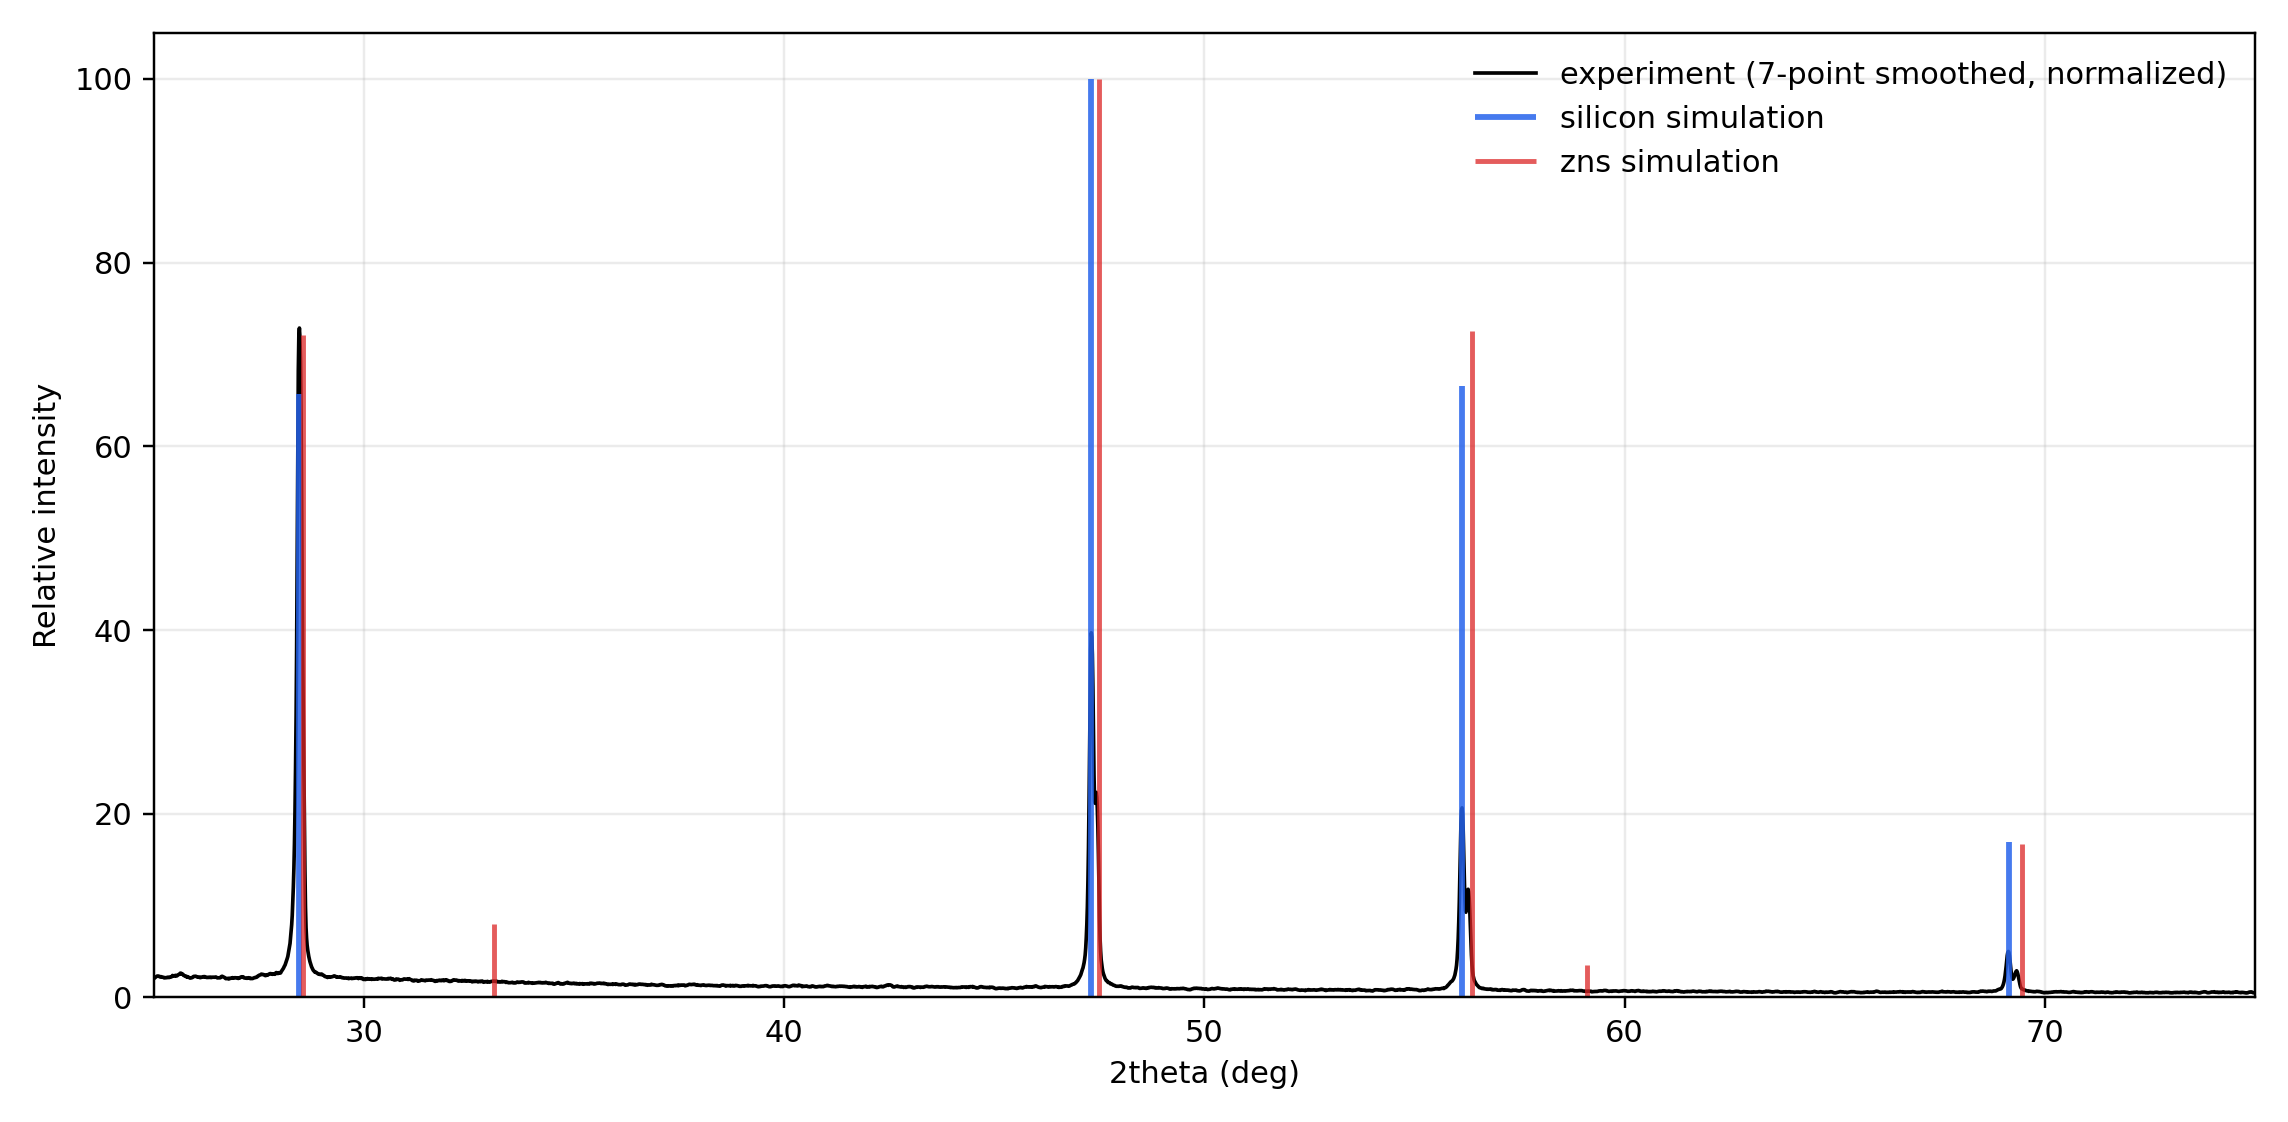
\includegraphics[width=0.92\textwidth]{figures/gr3_experiment_silicon_zns.png}
  \caption{Comparison of the experimental pattern with simulated AMCSD patterns for silicon and ZnS.}
  \label{fig:sim-comparisons}
\end{figure}

Silicon reproduces the observed strong peaks more accurately than ZnS. Its simulated reflections occur at \SI{28.445}{\degree}, \SI{47.308}{\degree}, \SI{56.129}{\degree}, and \SI{69.138}{\degree}, which are all very close to the experimental values. ZnS also reproduces the four strong peaks reasonably well, but its peaks are shifted slightly to higher $2\theta$ and it predicts weak additional reflections near \SI{33.09}{\degree} and \SI{59.12}{\degree}. A concrete similarity is that both simulations and the experiment share the strong peak near \SI{47.31}{\degree}. A concrete difference is that the ZnS simulation has a visible line near \SI{33.09}{\degree}, while the experimental data only show a marginal fluctuation in that region. This supports the interpretation that the sample is closer to silicon than to ZnS. The remaining differences in intensity can be explained by the simplified simulation, which does not include instrumental broadening, exact spectral splitting, preferred orientation, or full instrument-response effects.

\section{Discussion}
The dominant phase is best described as a cubic diamond-type phase. This conclusion is supported by the strong sequence of reflections $(111)$, $(220)$, $(311)$, and $(400)$ and by the lack of reliable peaks at \SI{33.32}{\degree} and \SI{59.16}{\degree}. The small local maxima in those regions should be treated as noise-level features rather than as established Bragg peaks.

Silicon and ZnS are both structurally relevant candidates, but silicon gives the better overall match. Its lattice parameter from the AMCSD entry, $a = \SI{5.4304}{\angstrom}$, is almost identical to the experimental value, and its allowed reflections match the observed strong peaks without requiring additional resolved peaks. ZnS remains useful as a comparison because its zinc-blende structure is closely related, but its extra weak reflections are less consistent with the data.

Pyrite was considered because some pyrite entries have lattice parameters close to the measured $a$, but it was rejected as the dominant phase because its simulated diffractogram contains several additional medium-to-strong reflections, especially near \SI{37}{\degree}, \SI{41}{\degree}, and \SI{51}{\degree}, that are not clearly resolved in the measured pattern. In this case, the overall reflection sequence is a stronger discriminator than closeness in lattice parameter alone.

\section{Conclusion}
The unknown powder was analyzed successfully as a cubic crystalline phase. From the strongest reflections, the unit-cell parameter was determined to be $a = \SI{5.4276}{\angstrom} = \SI{0.54276}{\nano\meter}$. The pattern is most consistent with a cubic diamond-type structure. Among the candidate models compared from the AMCSD, silicon is the most plausible identification, while ZnS serves as the main structural alternative. We are fairly confident about the cubic indexing and the lattice parameter, and more confident in silicon than in ZnS because the silicon peak positions agree more closely with the experiment and ZnS predicts weak extra reflections that are not clearly resolved in the measured data.

\section*{List of Symbols}
\begin{tabular}{ll}
$\lambda$ & wavelength of the X-rays \\
$\theta$ & diffraction angle \\
$2\theta$ & detector scan angle reported by the diffractogram \\
$d$ & interplanar spacing \\
$h,k,l$ & Miller indices \\
$a$ & cubic unit-cell parameter \\
$N$ & shorthand for $h^2+k^2+l^2$ \\
\si{\angstrom} & \SI{1}{\angstrom} = \SI{0.1}{\nano\meter} \\
\end{tabular}

\bibliographystyle{plainnat}
\bibliography{references}

\end{document}
